\documentclass[a4paper, 10pt]{article}

\usepackage[english]{babel}
\usepackage[utf8]{inputenc}
\usepackage{amsmath}
\usepackage{graphicx}
\usepackage[colorinlistoftodos]{todonotes}

\title{GODBases – Módulo de Banco de Dados Orientado a Objetos}

\author{Lucy Choque Mansilla ~~~~~~~ Silvia Scheunemann Silva\\
lucyacm@ime.usp.br ~~~~~~~~~~~~~~ silviass@ime.usp.br}

\graphicspath{{figures/}}

\begin{document}
\maketitle

\section{GODBases}

O módulo de banco de dados orientado a objetos (GODBases) foi elaborado com o intuito de compor o Projeto GOD e cumprir os requisitos da disciplina de Programação Orientada a Objetos. Tem por objetivo fornecer um banco de dados capaz de armazenar informações sobre o projeto GOD, possibilitando operações de inserção, remoção e busca. Seu desenvolvimento foi realizado no Squeak Smalltalk, através do banco de dados orientado a objetos, Magma.    


\subsection{Magma}
Magma é uma biblioteca de banco de dados orientado a objetos disponível no Squeak, no modo monousuário (single-user) e também multiusuário (arquitetura cliente-servidor). Os pacotes e métodos disponíveis podem ser obtidos através do download na página:
\begin{itemize}
\item{http://map.squeak.org/packagesbyname.}
\end{itemize}

\subsubsection{Instalação do magma}
Nesta seção são descritos os requisitos para instalação e instruções principais para trabalhar com a biblioteca.


Para o uso do magma, é recomendável a instalação de uma máquina virtual (Virtual Machine - VM) para lidar com problemas de sistema operacional na parte de persistência de informações (uso de imagens). De uma forma geral, a VM proporciona um ganho significativo de performance.

\begin{newpage}
\subsubsection{Passos de Instalação}

Um modo de instalar é usando o "SqueakMap Catalog" que está em "Apps" na barra de menu do Squeak (ver Fig.~\ref{fig:passo1_InstallMagma1}).

\begin{figure}[!htb]
\centering
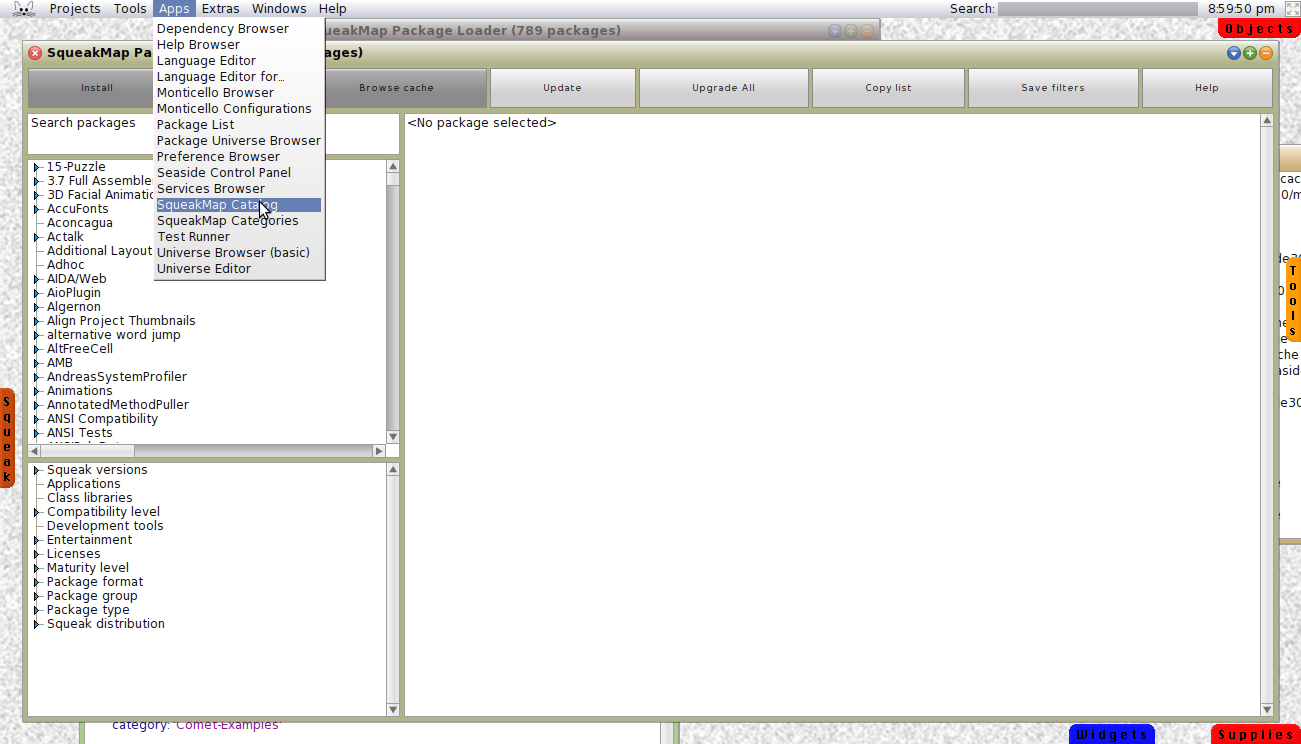
\includegraphics[width=0.7\textwidth]{passo1_InstallMagma1.png}
\caption{Instruções para instalação do magma.}
\label{fig:passo1_InstallMagma1}
\end{figure}

Logo, seguir os seguintes passos:
\begin{itemize}
\item{No SqueakMap clique com o botão direito do mouse no quadro esquerdo superior e garantir que todas as opções estejam desmarcadas. Isso permitirá visualizar os pacotes do Magma (Ver Fig.~\ref{fig:passo2_InstallMagma2}).}

\begin{figure}[!htb]
\centering
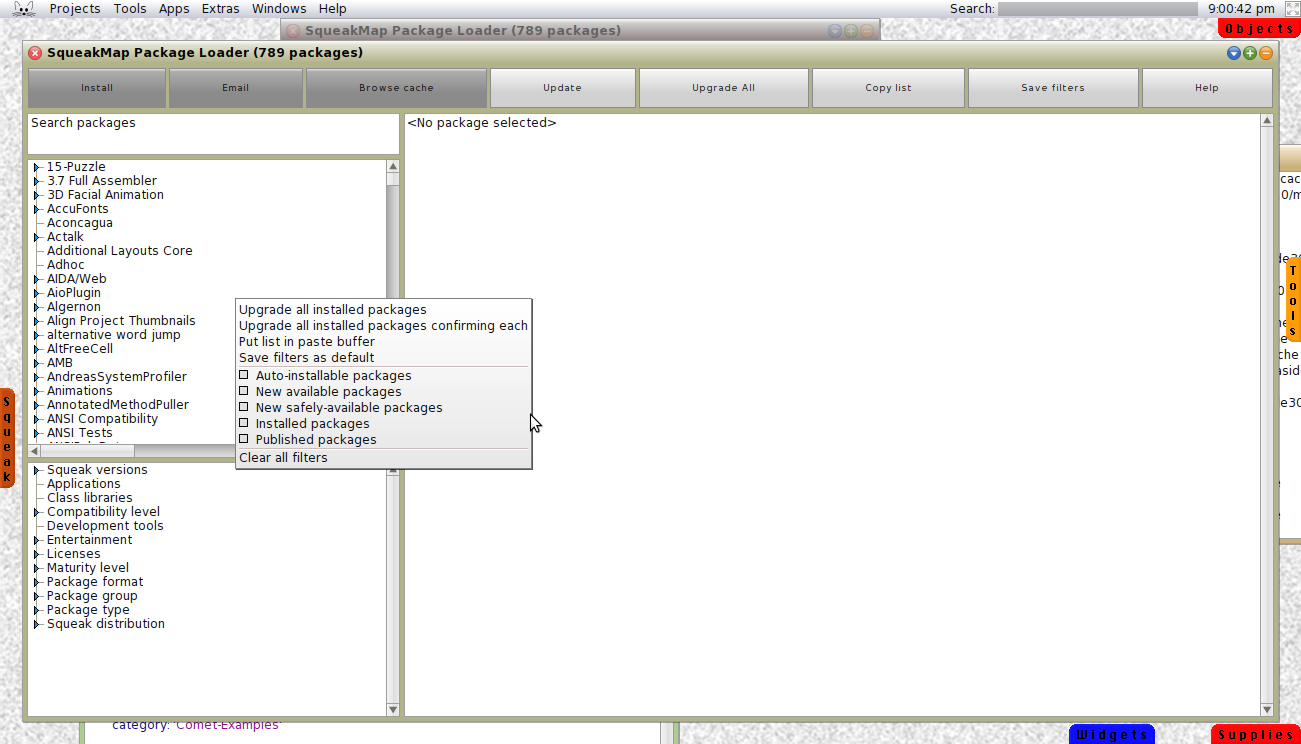
\includegraphics[width=0.7\textwidth]{passo2_InstallMagma2.png}
\caption{Instruções passo 2.}
\label{fig:passo2_InstallMagma2}
\end{figure}


\item{Clique com o botão direito do mouse no pacote "client" (versão 1.4) do Magma e escolher a opção "install".(Ver Fig.~\ref{fig:passo3_InstallMagmaClient})}

\begin{figure}[!htb]
\centering
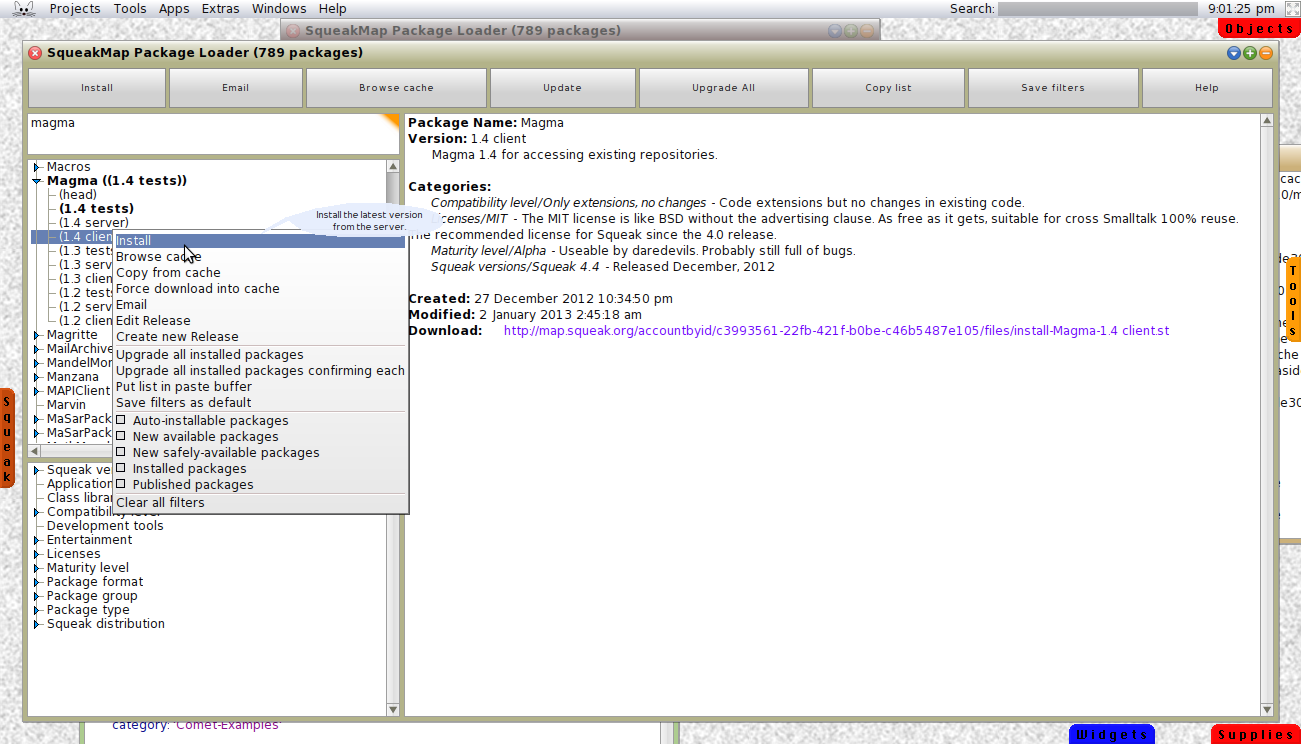
\includegraphics[width=0.8\textwidth]{passo3_InstallMagmaClient.png}
\caption{Instruções passo 3.}
\label{fig:passo3_InstallMagmaClient}
\end{figure}


\item{Repetir o ponto 2 para instalar os pacotes  "server" e o "test" do Magma. (Ver Fig.~\ref{fig:passo4_InstallMagmaServer})}

\begin{figure}[!htb]
\centering
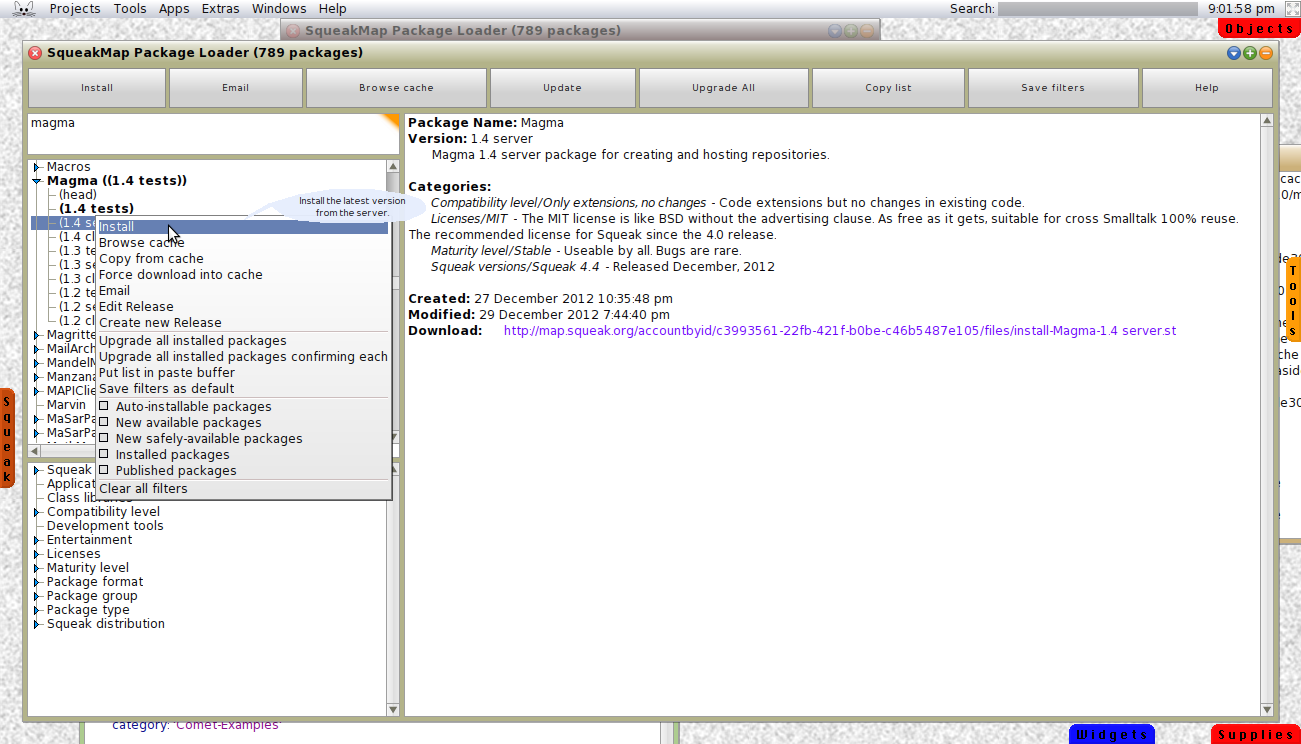
\includegraphics[width=0.8\textwidth]{passo4_InstallMagmaServer.png}
\caption{Instruções passo 4.}
\label{fig:passo4_InstallMagmaServer}
\end{figure}


\end{itemize}
\end{newpage}


\begin{newpage}
\subsection{ Classes do GODBases}
O pacote GODBases contém os principais métodos do banco de dados orientado a objetos do projeto GOD. A seguir fazemos uma pequena descrição sobre cada uma de suas classes.


\subsubsection{GDBServerController}

A classe GDBControllerServer permite fazer transações diferentes no servidor do banco de dados, bem como criar e eliminar um repositório. 

\begin{itemize}
\item Para criar um repositório padrão, execute a seguinte linha no workspace:\\
 { GDBServerController createRepository.}
\item Para criar um repositório especifico, execute:\\
{GDBServerController createRepository: 'nomeDoRepositorio'.}
\item Para inicializar o servidor com um repositório padrão, execute:\\
{GDBServerController startServer.}
\item Para inicializar o servidor com um repositório específico, execute:\\
{GDBServerController startServer:'nomeDoRepositorio'.}
\item{Para saber se o servidor foi iniciado, execute:}
{GDBServerController isStarted.}\\
esse comando retorna 'true' se o servidor estiver inicializado.
\end{itemize}

Uma vez inicializado o servidor, salve como uma imagem-servidor. Assim, para fechar o servidor, só precisa fechar a imagem salva, e quando você abri-lo novamente, o servidor já estará funcionando.

\begin{itemize}
\item Uma outra opção para fechar o servidor, é executar:\\
{GDBServerController stopServer.}
\item Para apagar um repositório específico, execute:\\
{GDBServerController deleteRepository:'nomeDoRepositorio'}
\end{itemize}


\subsubsection{GDBClientController}

A classe GDBClientController permite fazer a conexão de um usuário/ cliente com o servidor do banco de dados.
Primeiro é necessário inicializar o servidor em uma imagem separada, como indicado anteriormente, em seguida, executar as seguintes instruções:

\begin{itemize}
\item Para conectar um cliente com o banco de dados, execute o seguinte:\\
{GDBClientController initializeSession}
\end{itemize}

Uma vez inicializada a sessão do usuário é possível fazer qualquer transação no banco de dados, ou seja, é possível fazer uso dos métodos contidos nas classes: GDBDatabase, GDBData e GDBConference.


\begin{itemize}
\item Para atualizar qualquer alteração de outro cliente, antes de qualquer transação execute:\\
{GDBClientController refresh.}
\item Para alterar a sessão do cliente, execute o seguinte:\\
{GDBClientController refresh: 'nomeDeOutroCliente'.}
\end{itemize}

Uma vez que não se precise de fazer nenhuma transação a mais no banco de dados, só temos que desconectar a sessão do cliente, para isso execute o seguinte:\\
{GDBClientController release.}



\subsubsection{GDBDatabase}
A classe GDBDatabase permite criar o banco de dados. Nosso banco de dados é representado por um dicionário que armazena duas coleções, uma coleção do tipo MagmaCollection para armazenar os objetos GODData e uma outra do tipo OrderedCollection para armazenar uma coleção que contém objetos GCConference.\\

\begin{itemize}
\item Para criar o banco de dados, execute:\\
{GDBDatabase createDatabase}\\
\item Se você quiser criar apenas o banco de dados para armazenar objetos GODData, execute:\\
{GDBData createGODDataCollection.}\\
\item Se você quiser criar apenas o banco de dados para armazenar a coleção que vai conter objetos GCConference, execute:\\
{GDBConference createConferenceCollection.}
\end{itemize}

\subsubsection{GDBData}
A classe GDBData permite fazer transações diferentes no banco de dados para objetos GODData. 


\begin{itemize}
\item Para inserir um novo objeto GODData no banco de dados, execute:\\
{ GDBData add: meuGODData.}
\item Para remover um objeto GODData do banco de dados, execute:\\
{ GDBData remove: meuGODData.}
\item Para atualizar um objeto GODData por um outro objeto GODData, execute:\\
{ GDBData update: meuAntigoGODData with: meuNovoGODData.}
\item Se você quiser apagar todos os objetos GODData armazenados no banco de dados, execute:\\
{GDBData resetData.}

\item Para buscar um objeto GODData usando parte do nome do autor, execute:\\
{ GDBData searchAuthor: 'parteDoNomeDoAutor'.}
\item Para buscar um objeto GODData usando parte do nome do titulo, execute:\\
{ GDBData searchTitle: 'parteDoNomeDoTitulo'.}
\item Para buscar um objeto GODData usando um bloco, execute:\\
{ GDBData searchFor: umBloco.}\\
onde um bloco deve ter a forma:\\
$[:objeto | objeto atributoDoObjetoGODData = valorDeConparacaoParaABusca]$.

\item Para buscar um objeto GODData usando seu ID, execute:\\
{ GDBData searchById: umIdDoTipoInteiro.}
\item Para fazer uma busca exata pelo nome do autor, execute:\\
{ GDBData exactSearchByAuthor: 'nomeExatoDoAutor'.}
\item Para fazer uma busca exata pelo titulo, execute:\\
{ GDBData exactSearchByTitle: 'nomeExatoDoTitulo'.}	

\end{itemize}


\subsubsection{GDBConference}
A classe GDBConference permite fazer diferentes transações no banco de dados para objetos GCConference. 

\begin{itemize}
\item Para inserir uma nova coleção que armazena objetos GCConference, execute:\\
{GDBConference saveConferences: minhaColeçãoGCConference.}
\item Para recuperar essa coleção armazenada no banco de dados, execute:\\
{GDBConference loadConferences.}
\item Se você quiser apagar essa coleção armazenada no banco de dados, execute:\\
{GDBConference resetConferenceData.}
\end{itemize}

\end{newpage}


\end{document}